%\newpage
\section {Analysis Model}
\subsection {Data Flow diagram}
\vspace*{1.5cm}
\hspace{6.5cm} \textbf{Level 0}


\begin{figure}[H]
\centering
\setlength\fboxsep{0pt}
\setlength\fboxrule{0.5pt}
\fbox{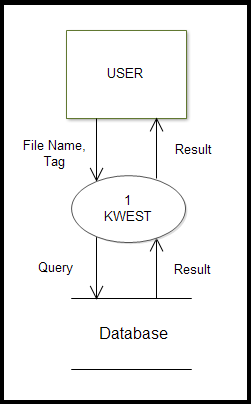
\includegraphics[width=0.5\linewidth]{./diagrams/dfd0.png}}
%\includegraphics[width=0.8\textwidth]{image.png}
\caption{Data flow diagram - Level 0}
\label{fig:dfd0}
\end{figure}

\newpage
\vspace*{2cm}
\hspace{5.5cm} \textbf{Level 1} \\
\begin{figure}[H]
\centering
\setlength\fboxsep{0pt}
\setlength\fboxrule{0.5pt}
\fbox{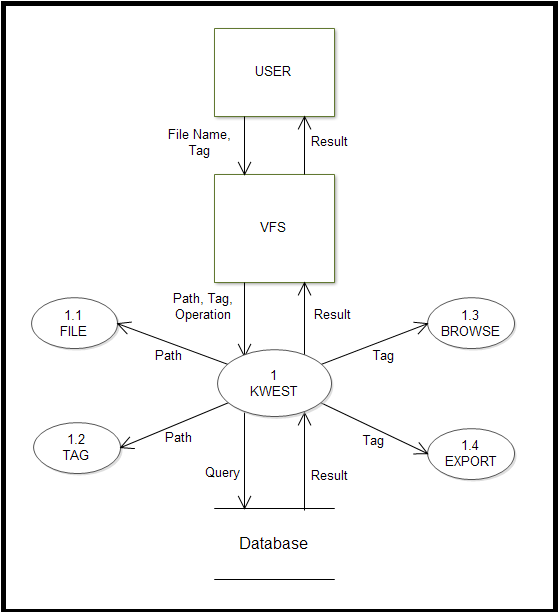
\includegraphics[width=0.9\linewidth]{./diagrams/dfd1.png}}
%\includegraphics[width=0.8\textwidth]{image.png}
\caption{Data flow diagram - Level 1}
\label{fig:dfd1}
\end{figure}

\newpage
\vspace*{2cm}
\hspace{5.5cm} \textbf{Level 2} \\
\begin{figure}[H]
\centering
\setlength\fboxsep{0pt}
\setlength\fboxrule{0.5pt}
\fbox{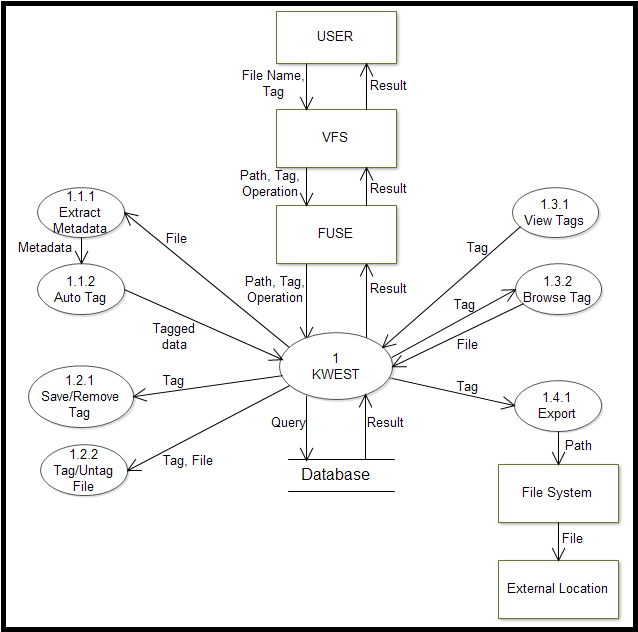
\includegraphics[width=0.9\linewidth]{./diagrams/dfd2.png}}
%\includegraphics[width=0.8\textwidth]{image.png}
\caption{Data flow diagram - Level 2}
\label{fig:dfd2}
\end{figure}

\newpage
\subsection {Entity Relationship diagram}
\begin{figure}[H]
\centering
\setlength\fboxsep{0pt}
\setlength\fboxrule{0.5pt}
\fbox{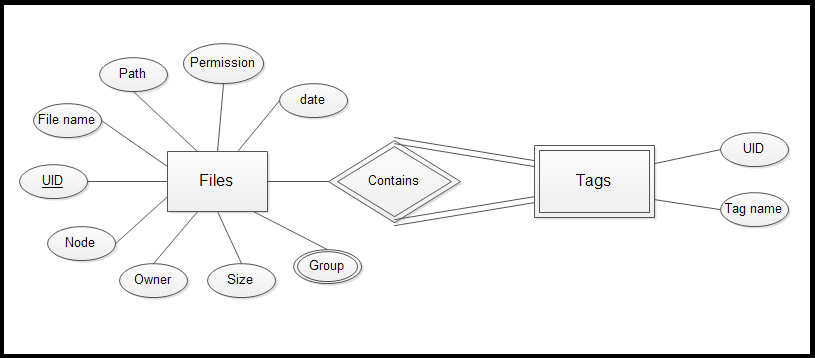
\includegraphics[width=0.8\linewidth]{./diagrams/ER.png}}
%\includegraphics[width=0.8\textwidth]{image.png}
\caption{Entity Relationship diagram}
\label{fig:ERdiag}
\end{figure}

